\documentclass[12pt,a4paper]{report}
\usepackage[top = 1.6cm, left = 2.7cm, right = 2.7cm ]{geometry}
\usepackage{setspace}
\usepackage[utf8]{inputenc}
\usepackage[francais]{babel}
\usepackage{float}
\usepackage[T1]{fontenc}
\usepackage{amsmath}
\usepackage{amsthm}
\usepackage{amsfonts}
\usepackage{amssymb}
\usepackage{graphicx}
\usepackage{hyperref}
\usepackage{thmtools}
\usepackage{cite}
\usepackage{bbm} 

%% Theorem Styles %%

\theoremstyle{definition}
\newtheorem{definition}{Définition}[chapter]
\newtheorem{propriete}{Propriété}[chapter]
\newtheorem*{proprietes}{Propriétés}
\theoremstyle{remark}
\newtheorem{example}{Exemple}[chapter]
\newtheorem{remark}{Remarque}[chapter]

%% Commandes persos %%
\newcommand\bbone{\ensuremath{\mathbbm{1}}}
\newcommand{\eg}{\textit{e.g.}}
\newcommand{\ssi}{\textit{ssi} }
\newcommand{\ie}{\textit{i.e.}, }
\newcommand{\cf}{\textit{cf.} }
\newcommand{\pr}{\mathbb{P}}
\renewcommand{\listtheoremname}{Définitions, propriétés et exemples}

\setstretch{1,1}
\let\labelitemi\labelitemii


\begin{document}
\begin{titlepage}
	
	\newcommand{\HRule}{\rule{\linewidth}{0.5mm}} % Defines a new command for the horizontal lines, change thickness here
	
	\center % Center everything on the page 
	%----------------------------------------------------------------------------------------
	%	HEADING SECTIONS
	%----------------------------------------------------------------------------------------
	
	\textsc{\LARGE Université de Mons}\\[1.5cm] % Name of your university/college
	\textsc{\Large Service d'informatique théorique }\\[0.5cm] % Major heading such as course name
	
	\vspace{1cm}
	%----------------------------------------------------------------------------------------
	%	TITLE SECTION
	%----------------------------------------------------------------------------------------
	
	\HRule \\[0.4cm]
	{ \huge \bfseries Jeux avec plus court chemin}\\[0.4cm] % Title of your document
	\HRule \\[1.5cm]
	
	%----------------------------------------------------------------------------------------
	%	AUTHOR SECTION//
	%----------------------------------------------------------------------------------------
	\vspace{2cm}
	\begin{minipage}{0.4\textwidth}
		\begin{flushleft} \large
			Projet de Master 1\\
			\emph{Auteur :} \\ \quad Florent Delgrange\\
		\end{flushleft}
	\end{minipage}
	~
	\begin{minipage}{0.4\textwidth}
		\begin{flushright} \large
			\emph{Directeurs:}\\ \quad Véronique Bruyère \\ \quad Mickaël Randour
		\end{flushright}
		
	\end{minipage}\\[5cm]
	
	% If you don't want a supervisor, uncomment the two lines below and remove the section above
	%\Large \emph{Author:}\\
	%John \textsc{Smith}\\[3cm] % Your name
	
	%----------------------------------------------------------------------------------------
	%	DATE SECTION
	%----------------------------------------------------------------------------------------
	\vspace{7cm}
	{\large \today}\\[3cm] % Date, change the \today to a set date if you want to be precise
	
	%----------------------------------------------------------------------------------------
	%	LOGO SECTION
	%----------------------------------------------------------------------------------------
	
	%\includegraphics{Logo}\\[1cm] % Include a department/university logo - this will require the graphicx package
	
	%----------------------------------------------------------------------------------------
	
	\vfill % Fill the rest of the page with whitespace
	
\end{titlepage}

\newpage
\tableofcontents
\listoftheorems[ignoreall,show={definition,example}]
\newpage

\chapter{Chaines de Markov}

Insérer ici une introduction aux chaines de Markov et une définition non-formelle.\\

Les définitions proposées dans ce chapitre sont inspirées du chapitre \textit{Probabilistic Systems} du livre \textit{Principles of model checking} ~\cite{DBLP:books/daglib/0020348}.

\section{Introduction aux probabilités}
Les chaines de Markov sont des automates qui modélisent des phénomènes aléatoires dont les transitions sont enrichies par des probabilités. Avant de définir strictement ce système, il est donc utile d'introduire brièvement quelques notions de probabilités qui seront indispensables à la compréhension de la suite du document.

\begin{definition}[\textbf{$\sigma$-algèbre}]
	Un $\sigma$-algèbre est une paire $(\Omega, \sigma)$ où $\Omega \neq \emptyset $ et $\sigma \subseteq \mathcal{P}(\Omega)$ qui respecte les $3$ conditions suivantes :
	\begin{enumerate}
		\item $\varnothing \in \sigma$
		\item Si $E \in \sigma$, alors $\overline{E} = \Omega \setminus E$ et $\overline{E} \in \sigma$
		\item Si $E_1, E_2, \dots \in \sigma$, alors $\bigcup_{n \geq 1} E_n \in \sigma$
	\end{enumerate}
	Les éléments de $\Omega$ sont appelés \textit{résultats} et les éléments de $\sigma$ sont appelés \textit{évènements}.
\end{definition}

\begin{remark}
	Ces conditions sur le $\sigma$-algèbre mènent au fait que $\overline{\Omega} = \varnothing$ implique $\Omega \in \sigma$.
\end{remark}
\begin{remark}[\textit{Cas particuliers}]
		$\sigma = \mathcal{P}(\Omega)$ signifie que tous les sous-ensembles de $\Omega$ sont des évènements et 
		$\sigma = \{\varnothing, \Omega\}$ signifie que $\forall E \subset \Omega$ tel que $E \neq \varnothing$, $E \notin \sigma$, \ie tout sous-ensemble non-vide de $\Omega$ n'est pas un évènement.
\end{remark}

\begin{definition}[\textbf{Mesure de probabilité}]\label{proba_measure} Soit $(\Omega, \sigma)$, un $\sigma$-algèbre.
	Une mesure de probabilité sur $(\Omega, \sigma)$ est une fonction $\mathbb{P} : \sigma \rightarrow [0, 1]$ tel que
	\begin{itemize}
		\renewcommand{\labelitemi}{\tiny$\bullet$}
		\item $\mathbb{P}(\Omega) = 1$
		\item Si $(E_n)_{n \geq 1}$ est une suite d'évènements disjoints $E_n \in \sigma$, alors:
		\[\mathbb{P}(\bigcup_{n \geq 1} E_n) = \sum_{n \geq 1} \mathbb{P}(E_n)\]
	\end{itemize}
	On dit alors que $(\Omega, \sigma, \mathbb{P})$ est un espace probabiliste.
	On appelle $\mathbb{P}(E)$ la mesure de probabilité de l'évènement $E$ ou encore plus simplement la probabilité de $E$.
\end{definition}

\begin{definition}[\textbf{Distribution de probabilité}]
	Soit $(\Omega, \sigma)$, un $\sigma$-algèbre. 
	On suppose que $\Omega$ est un ensemble dénombrable. Alors, $\exists \mu: \Omega \rightarrow [0,1]$, une mesure de probabilité telle que 
	\[\sum_{\omega \in \Omega} \mu(\omega) =1 \]
	$\mu$ est appelée \textit{distribution de probabilité sur $\Omega$}. Toute distribution induit une mesure de probabilité sur le $\sigma$-algèbre dont $\sigma = \mathcal{P}(\Omega)$ :
	\[ \forall E \in \sigma,\; \mathbb{P}_{\mu}(E) = \sum_{e \in E} \mu(e)\]
\end{definition}

\begin{proprietes}
	Soient $(\Omega, \sigma, \mathbb{P})$, un espace probabiliste.
	
	\begin{itemize}
		\renewcommand{\labelitemi}{\tiny$\bullet$}
		\item $\forall E \in \sigma$, $\mathbb{P}(E) = 1 - \mathbb{P}(\overline{E})$. En particulier, $\mathbb{P}(\varnothing) = 0$ (car $\mathbb{P}(\Omega) = 1$).
		\item \textit{(Les mesures de probabilité sont monotiques)} \[\forall E, E' \in \sigma \text{ tel que } E \subseteq E',\; \mathbb{P}(E') = \mathbb{P}(E) + \mathbb{P}(E' \setminus E) \geq \mathbb{P}(E)\]
		\item Soit $(E_n)_{n \geq 1}$, une suite d'évènements (pas forcément disjoints). \[\mathbb{P}(\bigcup_{n \geq 1} E_n) = \bigcup_{n \geq 1} E'_n \text{ où }E_1 = E'_1\text{ et }E'_n = E_n \setminus (E_1 \cup E_2 \cup \dots \cup E_{n-1}) \;\; \forall n \geq 2\]
		Par définition de $(E'_n)_{n \geq 1}$, on a toujours que $E'_n \cap E'_m = \varnothing$ quand $n \neq m$ (tous les éléments de la suite sont des ensembles disjoints), et donc que
		\[ \mathbb{P}(\bigcup_{n \geq 1} E_n) =  \mathbb{P}(\bigcup_{n \geq 1} E'_n) = \sum_{n \geq 1}\mathbb{P}(E'_n) \quad \text{\textit{(par déf. \ref{proba_measure})}}\]
		\item Soit $(E_n)_{n \geq 1}$, une suite d'évènements. Supposons que $E_1 \subseteq E_2 \subseteq E_3 \subseteq \dots $, alors, la monocité de $\mathbb{P}$ implique que $\mathbb{P}(E_1) \leq \mathbb{P}(E_2) \leq \dots \leq \mathbb{P}(E_n) \leq 1$.
		Supposons à présent que $E_1 \supseteq E_2 \supseteq E_3 \supseteq \dots$, alors :
		\[ \mathbb{P}(\bigcap_{n \geq 1}) = \lim_{n \rightarrow \infty} \mathbb{P}(E_n) \quad \text{\textit{(par la monocité)}}\]
	\end{itemize}
\end{proprietes}

\begin{example}[\textit{Lancer d'un dé}]
	On lance un dé. Chaque face a exactement une chance sur six d'apparaitre suite à ce lancer de dé. On défini strictement le $\sigma$-algèbre correspondant à ce lancer de dé : 
	Les résultats sont $\Omega = \{1, 2, 3, 4, 5, 6\}$ et les évènements sont $\sigma = \mathcal{P}(\Omega)$.
	On remarque que $\Omega$ est fini.
	De ce fait, on sait que $\exists \mu: \Omega \rightarrow [0,1]$ telle que $\mu$ est une distribution de probabilité
	où $\forall f \in \Omega, \; \mu(f) = \frac{1}{6}$.\\
	On est à présent intéressé par la probabilité des évènements suivants à l'aide de la mesure de probabilité $\pr$ induite par $\sigma$:
	\begin{itemize}
		\renewcommand{\labelitemi}{\tiny$\bullet$}
		\item "Le résultat du lancer de dé est 1 ou 6" = $\{1, 6\} \in \sigma$
		\[\pr(\{1,6\}) = \mu(1) + \mu(6) = \frac{1}{6} + \frac{1}{6} = \frac{1}{3}\]
		\item "Le résultat du lancer de dé n'est pas 1 ou 6" = $\overline{\{1, 6\}} = \{2, 3, 4, 5\}$
		\[\pr(\{2, 3, 4, 5\}) = 1 - \pr(\{1, 6\}) = 1 - \frac{1}{3} = \frac{2}{3}\]
	\end{itemize}
\end{example}

%\begin{example}[\textit{Lancers d'une pièce}]
%	On lance une infinité de fois une pièce. Le résultat d'un lancer de pièce est soit pile, soit face et la chance que le résultat de ce lancer de pièce soit pile est la même que le résultat soit face. L'ensemble des résultats $\Omega$ d'un lancer infini d'une pièce est donc l'ensemble des suites formées de pile ou de face, \ie, $\omega = \{x_1, x_2, \dots\} \in \Omega$ avec $x_n \in \{pile,\; face\} \;\; \forall n \in \mathbb{N}_0$. Cette fois, $\Omega$ est infini mais est toujours dénombrable. 
%\end{example}

\section{Définitions et propriétés}
\theoremstyle{definition}
\begin{definition}[\textbf{Chaine de Markov à temps discret}]
	
	Une \textit{chaine de Markov à temps discret}, notée \textbf{MC}, est un automate probabiliste défini par un tuple  $\mathcal{M} =$ (S, $\Delta$, $d_0$) où :
	\begin{itemize}
		\renewcommand{\labelitemi}{\tiny$\bullet$}
		\item $S$ est un ensemble dénombrable d'états. On dit que $\mathcal{M}$ est \textit{finie} \ssi $S$ est un ensemble fini.
		\item $\Delta: S \times S \rightarrow [0,1]$ est la \textit{fonction de probabilité de transition} telle que \[\forall s \in S, \sum_{s' \in S}\Delta(s, s')= 1\]
		%\item $d_0:S \rightarrow [0,1]$ est la distribution initiale telle que \[\sum_{s \in S}d_0(s)= 1\] (à noter que dans le cadre de ce document, la distribution initiale peut être omise, et dans ce cas, $\forall s \in S, d_0(s) = \frac{1}{|S|}$).
	\end{itemize}
\end{definition}

\begin{propriete}
	Les contraintes imposées sur $\Delta$ assurent que $\Delta$ est une distribution de probabilité sur $S$.
\end{propriete}
La fonction de probabilité de transition $\Delta$ spécifie pour tout état $s$ la probabilité de passer de cet état $s$ à l'état $s'$ en une étape (via une unique transition). 
%Plus strictement, soit $X_n$, une variable aléatoire représentant l'état du système après $n \in \mathbb{N}$ étapes, \[\Delta(s, s') = \mathbb{P}(X_{n+1} = s' | X_n = s) \]
$\Delta(s, s')$ est donc la probabilité que le système se trouve en l'état $s'$ à l'étape $n+1$ alors qu'il se trouvait en l'état $s$ à l'étape $n$. \\
%La valeur $d_0(s)$ spécifie la probabilité de commencer dans le système en l'état $s$. Si $d_0(s) > 0$, alors $s$ est appelé \textit{état initial}.% De la même manière, $d_0(s) = \mathbb{P}(X_0 = s)$.

\begin{definition}[\textbf{Graphe sous-jacent d'une chaine de Markov}]
	Une MC $\mathcal{M} = (S, \Delta)$ induit un \textit{graphe sous-jacent} (orienté) $G^\mathcal{M} = (V, E)$ où :
	\begin{itemize}
		\renewcommand{\labelitemi}{\tiny$\bullet$}
		\item $V$ est l'ensemble de sommets du graphe tel que $|V| = |S|$, \ie il existe une bijection de $S$ vers $V$. Chaque sommet $s' \in V$ est donc associé à un unique état $s \in S$. Par abus de langage, on dit que $V = S$.
		\item $E$ est l'ensemble des arcs du graphe tel que \[ \forall s, s' \in S, \; (s, s') \in E \text{ \ssi} \Delta(s, s') > 0\]
	\end{itemize}
\end{definition}

Afin d'illustrer une chaine de Markov, on utilise la représentation de son graphe sous-jacent où 
%\begin{itemize}
%	\renewcommand{\labelitemi}{\tiny$\bullet$}
%	 \item
chaque arc $(s, s') \in E$ est étiqueté par la probabilité de passer de l'état $s$ à l'état $s'$ en une étape : $\Delta(s, s')$.
	 %\item Si $\exists s, s' \in S$ tel que $d_0(s) \neq d_0(s')$, alors chaque état initial $s$ est illustré par un arc allant du vide vers le sommet $s$.
%\end{itemize}

\begin{example} [\textit{Simuler un lancé de dé avec une pièce de monnaie}] \label{knuthdie}
	On génère le comportement d'un dé via une pièce de monnaie selon l'algorithme probabiliste de Knuth et Yao ~\cite{KY76}. Cet algorithme est simulé à l'aide de la chaine de Markov $\mathcal{M}_{Kd}$ illustrée à la figure ~\ref{diebyacoin}. Lorsqu'on lance un dé, la probabilité de tomber sur n'importe quelle face du dé est exactement de $\frac{1}{6}$. Le comportement du système doit donc simuler ce phénomène lorsqu'un état final est atteint.
	\begin{figure}[H]
		\centering
		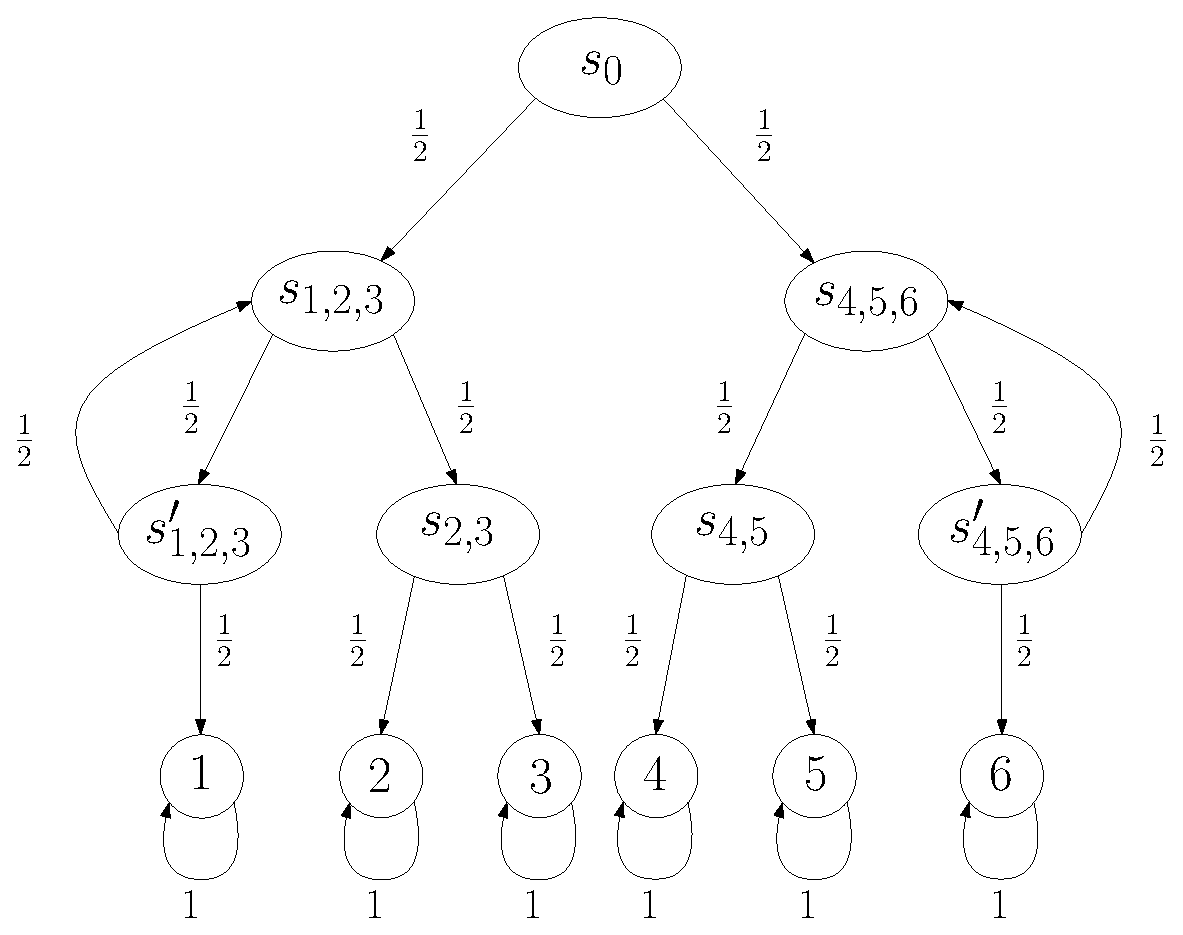
\includegraphics[scale=0.5]{figures/dieByaCoin.eps}
		\caption{Simulation d'un lancé de dé avec une pièce par une chaine de Markov}
		\label{diebyacoin}
	\end{figure}
	On commence en l'état $s_0$, qu'on appellera ici l'état initial. Les états $1, 2, 3, 4, 5, 6$ sont appelés états finaux et représentent les différentes faces du dé (\ie les résultats possibles du lancer de dé), tandis que les états internes ($\notin \{s_0, 1, 2, 3, 4, 5, 6\}$) représentent les états du système après un lancer de pièce. Pour tout état interne $\neq s_0$, un lancer de pièce dont le résultat est face emprunte l'arc de gauche pour déterminer son état suivant. Un lancer de pièce dont le résultat est pile emprunte l'arc de droite pour déterminer son état suivant.\\
	
	\textit{Simulation : }On suppose que le système démarre en l'état $s_0$. On lance une pièce. Si le résultat est face, le système évolue en l'état $s_{1, 2, 3}$. La probabilité que le résultat du lancer de pièce soit pile est égale à la probabilité que le résultat du lancer de pièce soit face. Par conséquent, en relançant la pièce, la probabilité que le système évolue en $s_{2, 3}$ est égale à la probabilité que le système évolue en $s'_{1, 2, 3}$. Si le système évolue en $s'_{1, 2, 3}$, un lancer de pièce mène à la face 1 du dé avec une probabilité $\frac{1}{2}$, égale à la probabilité de retourner en l'état $s_{1, 2, 3}$. Sinon, le système évolue en $s_{2, 3}$ et un lancer de pièce mènera obligatoirement au résultat d'un lancer de dé (avec une probabilité $\frac{1}{2} \text{ ou avec une probabilité }  \frac{1}{2}$, et donc avec une probabilité $1$), à savoir la face 2 ou 3. Le comportement du système se trouvant dans l'état $s_0$ dans le cas où le résultat du lancer de pièce est pile est symétrique.\\
	
	On verra plus tard dans ce document qu'en simulant un lancer de dé par une pièce, en suivant le système décrit par la MC $\mathcal{M}_{Kd}$ et en démarrant en l'état $s_0$, chaque face du dé est atteint avec une probabilité $\frac{1}{6}$.
\end{example}

\begin{definition}[\textbf{Matrice de transition}]
	Soient $\mathcal{M} = (S, \Delta)$, une MC finie et $n = |S|$. $S$ étant un ensemble fini. On peut dès lors énumérer les états de $S$. Soient $i,j \in \{1, \dots, n\}$ ($s_i \in S$, est le $i^{\text{ème}}$ sommet de $S$ et $s_j \in S$ est le $j^{\text{ème}}$ sommet de $S$).
	\textbf{P}$\in \mathbb{R}^{n \times n}$ est la matrice de transition de $\mathcal{M}$ \ssi $\textbf{P}_{i,j} = \Delta(s_i, s_j)$.\\
			 %\item $a^{(0)} \in \mathbb{R}^n$ est le vecteur initial de $\mathcal{M}$ \ssi $a^{(0)}_i = d_0(s_i)$
			%\end{itemize}
	La ligne $\textbf{P}_{i \cdot}$ contient la probabilité des transitions de l'état $s_i$ vers ses successeurs, tandis que la colonne $\textbf{P}_{\cdot j}$ spécifie la probabilité, pour tout état $s$, d'atteindre l'état $s_j$ en une étape.
\end{definition}

\begin{example}[\textit{Modèle d'Ehrenfest pour la diffusion des gaz}]
	Le modèle est proposé par Ehrenfest pour décrire les échanges de chaleur entre deux systèmes portés initialement à une température différente. On modélise la répartition de $N$ molécules de gaz à l'intérieur d'un récipient divisé en deux compartiments (urnes) séparés par une membrane poreuse.\\
	Pour cet exemple simplifié, on prend $N = 4$. Les 2 urnes contiennent $4$ molécules à tout moment et, à chaque étape, une des $4$ molécules est choisie au hasard et change d'urne (\cf figure ~\ref{ehrenfestscheme}).
	\begin{figure}[H]
		\centering
		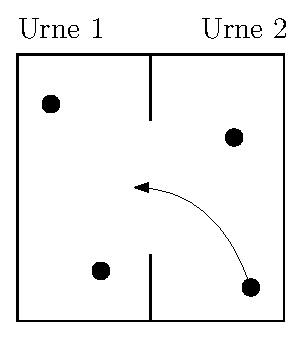
\includegraphics[scale=0.5]{figures/EhrenfestUrne.eps}
		\caption{Schéma simplifié du principe d'Ehrenfest pour $N=4$ molécules}
		\label{ehrenfestscheme}
	\end{figure}
	On modélise ce phénomène par une chaine de Markov (\cf figure ~\ref{ehrenfestMC}). Ici, $S=\{(2|2), (1|3), (0|4), (3|1), (4|0) \}$. Soit $s \in S$ 
	%tel que $s \neq (2|2)$, $d_0(s) = 0$, donc $(2|2)$ est l'unique état initial.
	Chaque état de $S$ correspond à la répartition des molécules dans les 2 urnes.
	\begin{figure}[H]
		\centering
		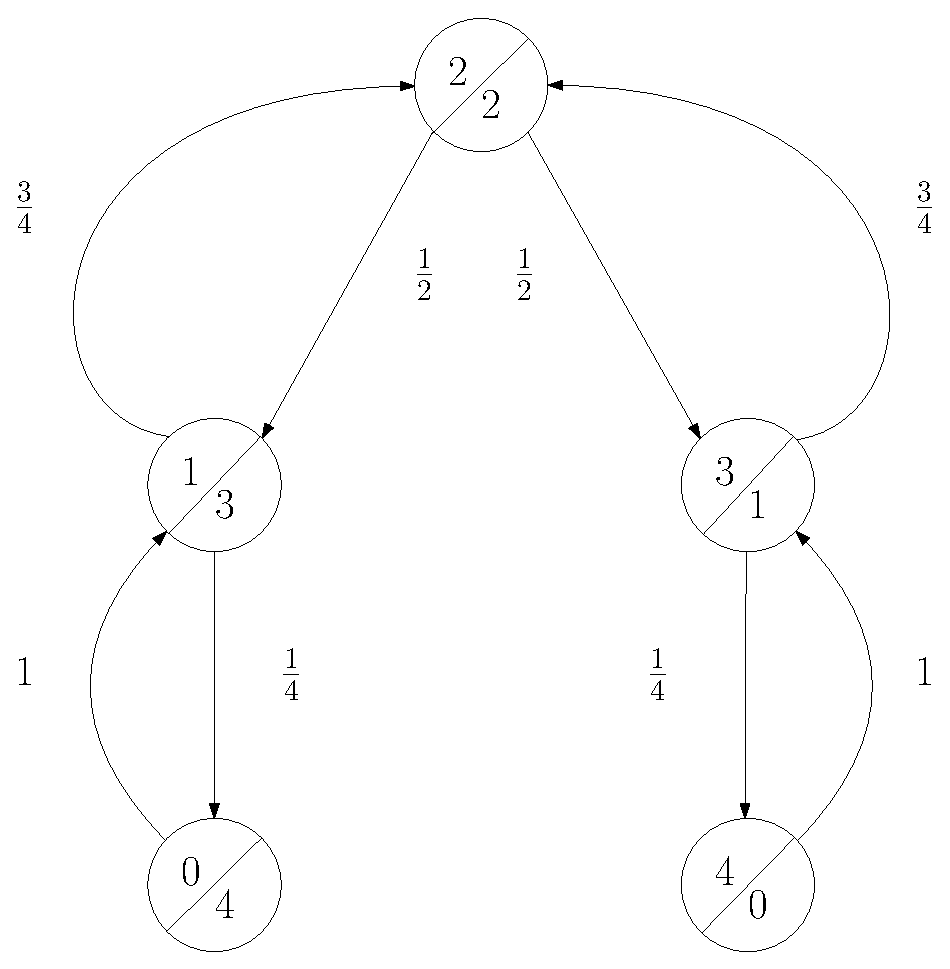
\includegraphics[scale=0.4]{figures/Ehrenfest.eps}
		\caption{Chaine de Markov associée pour $N=4$ molécules}
		\label{ehrenfestMC}
	\end{figure}
	En énumérant les état de $S$ comme suit : $(0|4), (1|3), (2|2), (3|1), (4|0)$, on a la matrice $5\times5$ de transition $\textbf{P}$:
	%et le vecteur initial $a^{(0)}$ 
	\[
		\textbf{P} =
			\begin{pmatrix}
			0 & 1 & 0 & 0 & 0 \\
			\frac{1}{4} & 0 & \frac{3}{4}& 0 & 0 \\
			0 & \frac{1}{2} & 0 & \frac{1}{2} & 0 \\
			0 & 0 & \frac{3}{4} & 0 & \frac{1}{4} \\
			0 & 0 & 0 & 1 & 0
			\end{pmatrix}
%			\\, \quad
%		a^{(0)} =
%			\begin{pmatrix}
%			0 \\ 0 \\ 1 \\ 0 \\ 0
%			\end{pmatrix}
	\]
\end{example}

\begin{definition}[\textbf{Chemin}]
	Soit $\mathcal{M} = (S, \Delta)$, une MC. On défini un \textit{chemin} $\pi$ de $\mathcal{M}$ comme étant une séquence d'états $\pi = s_0 s_1 s_2 \dots s_n$ tel que $\forall i \in \{0, \dots, n-1\}, s_i \in S$ et $\Delta(s_i, s_{i+1}) > 0$ (en d'autres termes, si l'arc $(s_i, s_{i+1}) \in E$ dans le graphe sous-jacent $G^\mathcal{M} = (S, E)$).% Le chemin est dit \textit{initial} si il commence en un état initial.
	\\
	On dénote par $\textit{Paths}(\mathcal{M})$ l'ensemble des \textit{chemins infinis}, \ie des séquences $s_0 s_1 s_2 \dots \in S^\omega$ tel que $\Delta(s_i, s_{i+1}) > 0 \;\;\forall i \geq 0$ et $\textit{Paths}_\textit{fin}(\mathcal{M})$, l'ensemble des chemins finis de $\mathcal{M}$.\\
	De la même façon, $\textit{Paths}(s)$ désigne l'ensemble des chemins infinis qui commencent en l'état $s \in S$ et $\textit{Paths}_\textit{fin}(s)$, l'ensemble des chemins finis qui commencent en l'état $s \in S$.
\end{definition}

Soit $\pi = s_0 s_1 \dots s_n$, un chemin de $\mathcal{M}$. Si l'état du système est en $s_0$, on peut utiliser la fonction de probabilité de transition $\Delta$ afin de déterminer la probabilité que le système emprunte le chemin $\pi$: 
\[ \Delta(\pi) = \Delta(s_0 s_1 \dots s_n) = \prod_{0 \leq i < n} \Delta(s_i, s_{i+1}) \]

\begin{example}[\textit{Chemins dans le système du dé de Knuth}]
	Pour cet exemple, on reprend la MC de l'exemple \ref{knuthdie}. Soit le chemin infini $\pi = s_0 s_{1,2,3} s'_{1, 2, 3} s_{1,2,3} s_{2,3} 2^\omega \in Paths(\mathcal{M}_{Kd})$.
	On suppose que l'état actuel du système est $s_0$. Alors, la probabilité que le système emprunte le chemin $\pi$ est $\Delta(\pi) = \Delta(s_0 s_{1,2,3} s'_{1, 2, 3} s_{1,2,3} s_{2,3} 2^\omega) = \frac{1}{2} \cdot \frac{1}{2} \cdot \frac{1}{2} \cdot \frac{1}{2} \cdot \frac{1}{2} \cdot 1 = \frac{1}{2^5} = \frac{1}{32}$
\end{example}

\section{Problème d'accessibilité}

L'un des problèmes les plus élémentaire de l'étude des systèmes modélisés par une chaîne de Markov est de déterminer la probabilité d'atteindre un sous ensemble $T$ d'états cibles du système. La résolution de ce problème est fortement liée à l'étude des problèmes que nous allons rencontrer par la suite dans ce document.

\subsection{\'Ennoncé du problème}
Soient $\mathcal{M} = (S, \Delta)$ une MC et $T \subseteq S$, un ensemble d'états cibles. On dénote par $\Diamond T$ l'évènement "atteindre au moins un état de $T$ via un chemin dans $\mathcal{M}$". Dès lors, soit $s \in S$, \[\mathbb{P}(s \models \Diamond T) = \mathbb{P}(\{\pi \in \textit{Paths}(s) | \pi \models \Diamond T\})\] est la probabilité qu'un chemin commençant en l'état $s$ satisfasse l'évènement $\Diamond T$, ou encore la probabilité d'atteindre un état de $T$ depuis l'état $s$ via un chemin dans $\mathcal{M}$.\\
On suppose que $x_s = \mathbb{P}(s \models \Diamond T)$ pour un $s \in S$ arbitraire. Alors, résoudre $x_s \; \forall s\in S$, revient à résoudre le problème d'accessibilité de la MC $\mathcal{M}$ pour $T$.
\subsection{Résolution du problème}
On va calculer $x_s$ $ \forall s \in S$.
\begin{enumerate}
	\item Si $T$ ne peut pas être atteint depuis le sommet $s$ dans le graphe sous-jacent $G^\mathcal{M}$, alors $x_s = 0$.
	\item Si $s \in T$, alors $x_s = 1$.
	\item Si $s \in S \setminus T$ et que $1.$ n'est pas vérifiée, alors 
		\[ x_s = \sum_{s' \in S \setminus T} \Delta(s, s') \cdot x_{s'} + \sum_{t \in T} \Delta(s, t) \]
\end{enumerate}

\begin{figure}[H]
	\centering
	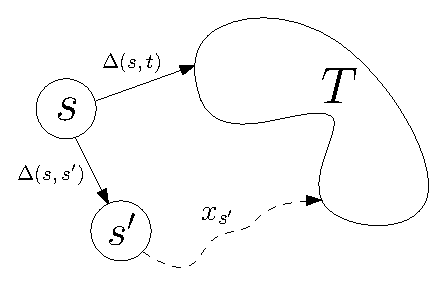
\includegraphics[scale=0.6]{figures/reachability.eps}
	%\caption{Illustration de l'accessibilité de l'état $s$ vers le sous-ensemble d'états $T$}
	\label{reachablity}
\end{figure}

\begin{itemize}
\renewcommand{\labelitemi}{\tiny$\bullet$}
	\item $ \sum_{s' \in S \setminus T}  \Delta(s, s') \cdot x_{s'} $ correspond à la probabilité que $s$ atteigne le sous-ensemble d'états $T$ en passant par un état intermédiaire $s' \in S \setminus T$.
	\item $\sum_{t \in T} \Delta(s, t)$ correspond à la probabilité que $s$ atteigne le sous-ensemble d'états $T$ en une seule étape.
\end{itemize}
Soit $n = |S|$. On obtient alors un système de $n$ équations à $n$ inconnues.

\begin{example}[\textit{Problème d'accessibilité}]\label{reachex}
	On considère la chaine de Markov $\mathcal{M}_{re} = (S, \Delta)$ de la figure \ref{reachability-example} tel que $S = \{s_0, s_1, s_2, s_3, s_4, s_5, s_6\}$ et $T \subseteq S$ tel que $T = \{ s_5, s_6 \}$. On est intéressé par $\mathbb{P}(s \models \Diamond T) \; \forall s \in S$.
	\begin{figure}[H]
	\centering
	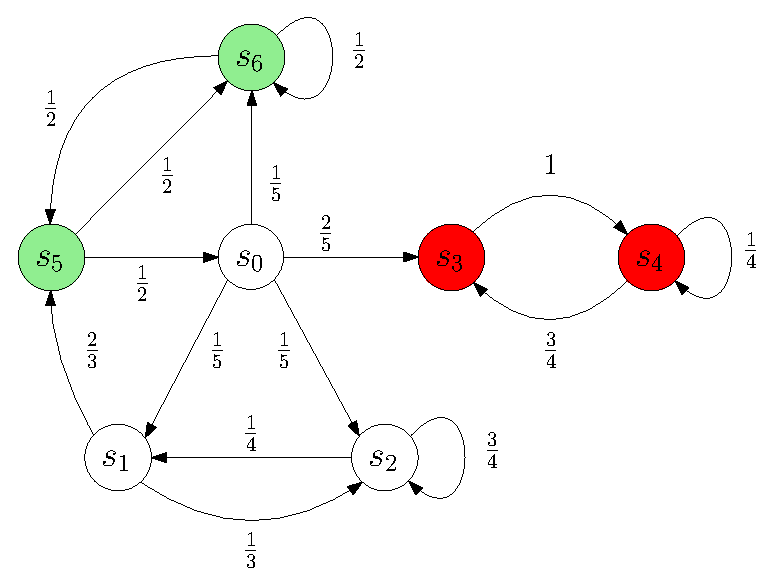
\includegraphics[scale=0.7]{figures/reachability-example.eps}
	\caption{Chaine de Markov sur laquelle on va résoudre le problème d'accessibilité}
	\label{reachability-example}
	\end{figure}

Par le fait que $T = \{s_5, s_6\}$, on a que $x_{s_5} = x_{s_6} = 1$. Le graphe sous-jacent $G^{\mathcal{M}_{re}}$ permet de détecter que %la sous-chaine absorbante composée des états $s_3$ et $s_4$ n'atteint jamais %
les états $s_3$ et $s_4$ n'atteignent jamais un état de $T$. Dès lors, on a que $x_{s_3} = x_{s_4} = 0$.
\[
	\begin{cases}
		x_{s_0} = \frac{1}{5} x_{s_1} + \frac{1}{5} x_{s_2} + \frac{2}{5} x_{s_3} + \frac{1}{5} \\
		x_{s_1} = \frac{1}{3} x_{s_2} + \frac{2}{3} \\
		x_{s_2} = \frac{1}{4} x_{s_1} + \frac{3}{4} x_{s_2} \\
		x_{s_3} = 0 \\
		x_{s_4} = 0 \\
		x_{s_5} = 1 \\
		x_{s_6} = 1
	\end{cases}
	\iff
	\begin{cases}
	x_{s_0} - \frac{1}{5} x_{s_1} - \frac{1}{5} x_{s_2} - \frac{2}{5} x_{s_3} = \frac{1}{5} \\
	x_{s_1} - \frac{1}{3} x_{s_2} = \frac{2}{3} \\
	\frac{-1}{4} x_{s_1} + \frac{1}{4} x_{s_2} = 0 \\
	x_{s_3} = 0 \\
	x_{s_4} = 0 \\
	x_{s_5} = 1 \\
	x_{s_6} = 1 
	\end{cases}
\]

Afin de résoudre ce système, il est utile de le passer sous forme matricielle :

\[
\begin{pmatrix}
1 & \frac{-1}{5} & \frac{1}{5} & \frac{-2}{5} & 0 & 0 & 0 \\[0.3em]
0 & 1 & \frac{-1}{3} & 0 & 0 & 0 & 0 \\[0.3em]
0 & \frac{-1}{4} & \frac{1}{4} & 0 & 0 & 0 & 0 \\[0.3em]
0 & 0 & 0 & 1 & 0 & 0 & 0 \\[0.3em]
0 & 0 & 0 & 0 & 1 & 0 & 0 \\[0.3em]
0 & 0 & 0 & 0 & 0 & 1 & 0 \\[0.3em]
0 & 0 & 0 & 0 & 0 & 0 & 1
\end{pmatrix}
\;
\begin{pmatrix}
x_{s_0} \\[0.3em] x _{s_1} \\[0.3em] x_{s_2} \\[0.3em] x_{s_3} \\[0.3em] x_{s_4} \\[0.3em] x_{s_5} \\[0.3em] x_{s_6}
\end{pmatrix}
 = \;
\begin{pmatrix}
\; \frac{1}{5} \\[0.3em] \frac{2}{3} \\[0.3em] 0 \\[0.3em] 0 \\[0.3em] 0 \\[0.3em] 1 \\[0.3em] 1
\end{pmatrix}
\]

Ce système d'équations linéaires peut se résoudre par la méthode du \textit{pivot de Gauss}. %insérer ref cours d'anum de troest%
Dès lors, la solution de ce système est :
\[
	x_{s_0} = \frac{1}{5}, \; x_{s_1} = 1, \; x_{s_2} = 1, \; x_{s_3} = 0, \; x_{s_4} = 0, \; x_{s_5} = 1, \; x_{s_6} = 1
\]
\end{example}

\begin{example}[\textit{Retour sur le dé de Knuth}]
	Reprenons la MC $\mathcal{M}_{Kd} = (S, \Delta)$ de l'exemple ~\ref{knuthdie}. Lorsqu'on lance un dé à $6$ faces, la probabilité d'obtenir n'importe quelle face de ce dé est de $\frac{1}{6}$. Dans $\mathcal{M}_{Kd}$, $s_0$ doit atteindre un des états finaux avec une probabilité $\frac{1}{6}$. On est donc intéressé de résoudre \[\mathbb{P}(s_0 \models \Diamond T) \;\; \forall T \in \{\{1\},\{2\},\{3\},\{4\},\{5\},\{6\}\} \]
	\`A l'aide du système défini dans cette sous-section, on calcule :
	\begin{spacing}{1.5}
	\begin{enumerate}
		\item $\mathbb{P}(s_0 \models \Diamond \{1\})$
		\begin{itemize}
			\renewcommand{\labelitemi}{\tiny$\bullet$}
			\item $x_1 = 1 $ car $1$ est l'état cible.
			\item $x_{s_{2, 3}} = x_{s_{4, 5, 6}} = x_{s_{4, 5}} = x_{s'_{4, 5, 6}} = x_2 = x_3 = x_4 = x_5 = x_6 = 0$ car ces sommets n'atteignent pas le sommet $1$ dans le graphe sous-jacent $G^{\mathcal{M}_{Kd}}$.
			\item $x_{s'_{1, 2, 3}} = \frac{1}{2} x_{s_{1, 2, 3}} + \frac{1}{2}$
			\item $x_{s_{1, 2, 3}} = \frac{1}{2} x_{s'_{1, 2, 3}} + \frac{1}{2}x_{s_{2, 3}} = \frac{1}{2} x_{s'_{1, 2, 3}} = \frac{1}{4} (x_{s_{1, 2, 3}} + 1) \Leftrightarrow
			4 x_{s_{1, 2, 3}} =x_{s_{1, 2, 3}} + 1 \Leftrightarrow x_{s_{1, 2, 3}} = \frac{1}{3}$
			%\item $x_{s'_{1, 2, 3}} = \frac{1}{6} + \frac{1}{2} = \frac{2}{3}$
			\item $x_{s_0} = \frac{1}{2} x_{s_{1,2,3}} + \frac{1}{2} x_{s_{4, 5, 6}} = \frac{1}{2} x_{s_{1,2,3}} = \frac{1}{6}$
		\end{itemize}
		\item $\mathbb{P}(s_0 \models \Diamond \{2\})$
		\begin{itemize}
			\renewcommand{\labelitemi}{\tiny$\bullet$}
			\item $x_2 = 1 $ car $2$ est l'état cible.
			\item $x_{s_{4, 5, 6}} = x_{s_{4, 5}} = x_{s'_{4, 5, 6}} = x_1 = x_3 = x_4 = x_5 = x_6 = 0$ car ces sommets n'atteignent pas le sommet $2$ dans le graphe sous-jacent $G^{\mathcal{M}_{Kd}}$.
			\item $x_{s_{2, 3}} = \frac{1}{2} x_{s_3}  + \frac{1}{2} = \frac{1}{2} x_{s_2}$
			\item $x_{s'_{1, 2, 3}} = \frac{1}{2} x_{s_{1, 2, 3}} + \frac{1}{2} x_{s_1} = \frac{1}{2} x_{s_{1, 2, 3}}$
			\item $x_{s_{1, 2, 3}} = \frac{1}{2} x_{s'_{1, 2, 3}} + \frac{1}{2}  = 
			\frac{1}{2} (\frac{1}{2} x_{s_{1, 2, 3}}) +\frac{1}{2} (\frac{1}{2})
			= \frac{1}{4} x_{s_{1, 2, 3}} +\frac{1}{4}
			\Leftrightarrow \frac{3}{4} x_{s_{1, 2, 3}} = \frac{1}{4}
			\Leftrightarrow x_{s_{1, 2, 3}} = \frac{1}{3}$
			%\item $x_{s'_{1, 2, 3}} = \frac{1}{6} + \frac{1}{2} = \frac{2}{3}$
			\item $x_{s_0} = \frac{1}{2} x_{s_{1,2,3}} + \frac{1}{2} x_{s_{4, 5, 6}} = \frac{1}{2} x_{s_{1,2,3}} = \frac{1}{6}$
		\end{itemize}
		\item $\mathbb{P}(s_0 \models \Diamond \{3\}) = \frac{1}{6}$ (idem que $2.$).
	\end{enumerate}\end{spacing}
	Le comportement du système dans le cas où l'arc de droite est emprunté (\ie le résultat du premier lancer de pièce est pile) en $s_0$ est symétrique au cas où l'arc de gauche est emprunté (\cf exemple  ~\ref{knuthdie}). Dès lors, $\mathbb{P}(s_0 \models \Diamond \{4\}) = \mathbb{P}(s_0 \models \Diamond \{3\}) = \frac{1}{6}$ et $\mathbb{P}(s_0 \models \Diamond \{5\}) = \mathbb{P}(s_0 \models \Diamond \{2\}) = \frac{1}{6}$ et $\mathbb{P}(s_0 \models \Diamond \{6\}) = \mathbb{P}(s_0 \models \Diamond \{1\}) = \frac{1}{6}$. On a donc bien que le système simule un lancé de dé.
	
\end{example}

\subsection{Généralisation matricielle}
Le problème d'accessibilité pour la chaine de Markov $\mathcal{M} = (S, \Delta)$ et le sous-ensemble d'états cibles $T \subseteq S$ se résout par un système de $n$ équations à $n$ inconnues. Il est donc utile, comme nous l'avons vu dans l'exemple ~\ref{reachex} , de définir un système matriciel équivalent. \\
Soient $n' = |S \setminus T|$, $i, j \in \{1 \dots n'\}$, et $s_i, s_j$ les $i^{\text{ème}} \text{ et } j^{\text{ème}} $ sommets de $S \setminus T$. 
\begin{itemize}
\renewcommand{\labelitemi}{\tiny$\bullet$}
\item Soit $A \in \mathbb{R}^{n' \times n'}$, la matrice de probabilité de transitions tel que $(Ax)_{i}$ indique la probabilité que $s_i$ atteigne $T$ via un état intermédiaire. Alors, $A_{i,j} = \Delta(s_i, s_j)$.
\item Soit $b \in \mathbb{R}^{n'}$ tel que $b_{i}$ est la probabilité que $s_i$ atteigne $T$ en une étape. Alors, $b_i = \sum_{t \in T} \Delta(s_i, t)$.
\end{itemize}
Le système matriciel correspondant est
\[ x = Ax + b \]
Cette équation peut être réécrite sous forme d'un système d'équations linéaires
\[ (\mathbbm{1} - A) x = b \]
avec $\mathbbm{1}$, la matrice unité de cardinalité $n' \times n'$ dans le but de le résoudre avec des algorithmes de résolution de systèmes d'équations linéaires (\eg $\;$avec le pivot de Gauss).

%%% SOUS CHAINE ABSORBANTE ? %%%
\subsection{Classe Finale}
\begin{definition}[\textbf{\'Etat absorbant}]
	Soit $\mathcal{M} = (S, \Delta)$, une MC. $s \in S$ est un état absorbant de $\mathcal{M}$ \ssi $\Delta(s, s) = 1$.
\end{definition}

\begin{definition}[\textbf{Composante fortement connexe d'un graphe}]
	Soit $G=(V, E)$, un graphe orienté dont $V$ est l'ensemble de sommets de $G$ et $E$ est l'ensemble des arcs de $G$. $B \subseteq V$ est une composante fortement connexe de $G$ \ssi $\forall s,s' \in B,$ il existe un chemin $\pi = s_0 s_1 \dots s_n$ de $s$ à $s'$ tel que $s = s_0 , s' = s_n$ et $\forall i \in \{0 \dots n\}, s_i \in B$.
\end{definition}

\begin{definition}[\textbf{Classe finale}]
	Soient $\mathcal{M} = (S, \Delta)$, une MC et $B \subseteq S$. Le sous-ensemble $B$ est une classe finale de $\mathcal{M}$ \ssi $B$ est une composante fortement connexe de $G^\mathcal{M}$ et qu'aucun état en dehors de $B$ ne peut être atteint, \ie
	\[\forall b \in B, \sum_{b' \in B} \Delta(b, b') = 1 \iff \sum_{s \in S \setminus B} \Delta(b, s) = 0\]
\end{definition}

\begin{propriete}
		Soient $\mathcal{M}=(S, \Delta)$, une MC et $s \in S$ un état absorbant. L'ensemble $\{s\}$ est une classe finale de $\mathcal{M}$.
\end{propriete}

\begin{propriete}\label{BSCC-tip1}
	Soient $\mathcal{M} = (S, \Delta)$, une MC et $T \subseteq S$, un ensemble d'états cibles. On suppose que les états de $B \subseteq S$ forment une classe finale de $\mathcal{M}$ et que $T \cap B = \emptyset$. Alors, $\forall b \in B, \; \mathbb{P}(b \models \Diamond T) = 0$.
\end{propriete}

\textit{Application de la propriété ~\ref{BSCC-tip1} : } Soient $\mathcal{M} = (S, \Delta)$, une MC et $T \subseteq S$ un ensemble d'états cibles. On suppose que $B \subseteq S$ est une classe finale de $\mathcal{M}$ et que $T \cap B = \emptyset$. On construit la MC $\mathcal{M}' = (S', \Delta')$ où 
\begin{itemize}
\renewcommand{\labelitemi}{\tiny$\bullet$}
\item $S' = \{s^*\} \cup S \setminus B$
\item $s^*$ est un état absorbant
\item $\forall s, s' \in S' \setminus \{s^*\}, \; \Delta'(s, s') = \Delta(s, s')$
\item $ \forall s \in S', \Delta'(s, s^*) = \sum_{b \in B} \Delta(s, b)$
\end{itemize}
Alors, résoudre le problème d'accessibilité de $\mathcal{M}$ pour $T$ revient à résoudre le problème d'accessibilité de $\mathcal{M}'$ pour $T$. On dit que $\mathcal{M'}$ est induite par $B$.\\
	
\begin{example}[\textit{Classe finale}]
	Soient $\mathcal{M}_{re} = (S, \Delta)$, la MC de la figure \ref{reachability-example} et $T = \{s_5, s_6\}$, un ensemble d'états cibles. On a que les états $s_3$ et $s_4$ forment une classe finale de $\mathcal{M}_{re}$. La MC $\mathcal{M'}_{re}$ induite par cette classe finale est représentée à la figure ~\ref{absorbing-chain}
		\begin{figure}[H]
		\centering
		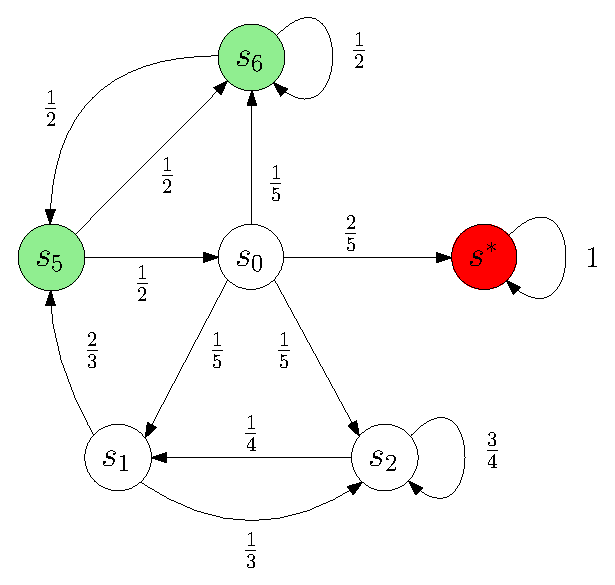
\includegraphics[scale=0.7]{figures/absorbing-chain.eps}
		\caption{Chaine de Markov induite par la sous-chaine absorbante formée par $s_3$ et $s_4$.}
		\label{absorbing-chain}
	\end{figure}
\end{example}


\bibliography{bib}{}
\bibliographystyle{plain}

\end{document}